In this chapter the client and it's functions are described. The Client exists of the following subsystems:
\begin{shortlist}
    \item MQTT
    \item Message/Config Parser
    \item Audio driver
    \item Relative Weight Factor
    \item Logger
\end{shortlist}

The aforementioned parts will be described in the following sections.

\section{MQTT}

The client uses the \href{http://mosquitto.org/}{Mosquitto MQTT C++ library}.
This is an open source client that implements the MQTT protocol versions 3.1 and 3.1.1.
MQTT is a publish-subscribe based \say{light weight} messaging protocol for use on top of the TCP/IP protocol.
It is designed for connections with remote locations where a \say{small code footprint} is required or the network bandwidth is limited.
This makes it suitable for \say{Internet of Things} messaging.

The client and the website use topics to communicate. The topics for the communication are described in the previous chapter.
The DNS class has a public inheritance of the Mosquito class.
This means all public and protected members of the Mosquitto class can be accessed by the DNS class.
The private members cannot directly accessed by DNS class. In the DNS class the Mosquitto functions are been overwritten by DNS's own implementation.
The Mosquitto functions are automatically called by the Mosquitto library.

If the client is executed the Mosquitto library calls the function
\textbf{ on connect}. This function published the client-id in the \textbf{online topic } and subscribe itself on the following topics:
\small{
\begin{itemize} [noitemsep, nolistsep]
	\item \textbf {request online}
	\item \textbf {request client data}
	\item \textbf {clients data}
	\item \textbf {music volume}
	\item \textbf {music status}
	\item \textbf {music sources}
\end{itemize}
}

If the client is stopped or disconnected the Mosquitto library calls the function \textbf {on disconnect}. This function published the client-id in the \textbf {offline topic}.\\

When the client is running and has excuted the function \textbf {on connect}, It waits on a message from a subscribed topic. If a message appears, the function \textbf {on message} is called. This function takes as parameters a mosquitto message struct, containing:
\small{
\begin{itemize} [noitemsep, nolistsep]
	\item \textbf {int mid}
	\item \textbf {char *topic}
	\item \textbf {void* payload}
	\item \textbf {int payloadlen}
	\item \textbf {int qos}
	\item \textbf {bool retain\\}
\end{itemize}
}

In the function is decided on which topic the message came from, by comparing the \textbf {topic} field with the topics defined in \ref{topics}. A list of actions is implemented for each topic.\\

MQTT has a funcion that is called \textbf {last will}. This function is called when a client times out, for example if the systems power cuts out and doesn't properly shutdown. The broker will detect this and publish the clients' last will message. In the client this function is used to publish its message to the \textbf {offline} topic.

\section{Message/Config Parser}

A large portion of the messages that are send in this application are in \href{http://www.json.org/}{JSON string format}. Since the C++ spec does not include a JSON Parser, the \href{https://github.com/Zguy/Jzon}{library JZON} is used to parse/compose the JSON string formats.\\

\subsection{Config}
The user must provide the client with a config file in JSON format which is used to initialize the client. The data that can be specified includes:
\small{
\begin{itemize} [noitemsep, nolistsep]
	\item \textbf {Name}
	\item \textbf {Log settings}
	\item \textbf {Topic prefix}
	\item \textbf {Broker}
	\item \textbf {Topics\\}
\end{itemize}
}
It should be noted that the config file has a \say{.js} extension, this is because the same config is also used by the website. The benefits of doing this is that you only have to change a single config file and everything adapts, instead of changing every client individually.

\subsection{Message}
The messages that are supplied in JSON format, are parsed using an iterative feature, ensuring full dynamic behavior. As an example, the message format of \say{info/clients/data/+} as specified in \ref{topics}:
\begin{lstlisting}
{
  "clientid1": {
    "objectid1": {
      "distance": 0,
      "angle": 0
    }
  },
  "clientid2": {
    "objectid1": {
      "distance": 0,
      "angle": 0
    },
    "objectid2": {
      "distance": 0,
      "angle": 0
    }
  },
  "clientid_n": {
    "objectid2": {
      "distance": 0,
      "angle": 0
    }
  }
\end{lstlisting}

This message can have any amount \say{n} of client-nodes, each containing any number \say{m} of objects-nodes. Jzon implements an iterator for JSON nodes, these can be used with C++14's great ranged based for loops. This allows the client to convert the JSON message into an map of objects per client, and a vector with all the distances, which in turn are used by the RWF calculations which will be touched on later.

\section{Audio driver}
\label{sec:client_audio_driver}

Since this project requires the client to play audio files, a small class was implemented to do just that. To keep development time low, a couple of cli tools were used to achieve functionality: vorbis tools' \texttt{ogg123} and pulse audio's \texttt{pactl}. An instance of this class is created for each audio object.
Playing the audio is straight forward, execute an instance of \texttt{ogg123} with a file path and save the PID. If the music has to be stopped (as per user input) simply call \texttt{kill([pid])} and the music stops playing.
The volume regulation is less straight forward. It uses \texttt{pactl list sink-inputs} to list all applications using pulse audio as output. This list is indexed and contains information such as application name, and process ID. So a loop checks each index in the list for the \texttt{ogg123} PID. Once the correct index has been found, it can then be used to set the stream volume with \texttt{pactl set-sink-input-volume [index] [volume]}.

\section{Relative Weight Factor}
\label{sec:client_relative_weight_factor}

This system is based on a virtual object that will create sound like it is in some 2D space.
This library calculates the volume level that a speaker needs to be in comparison with all the other speakers relative from an object.

\subsection{The problem}
\label{sub:client_rwf_the_problem}

To explain the inner workings lets look at an example.
In figure \ref{fig:client_rwf_center} is a simple setup. Two speakers \say{Sp1} and \say{Sp2}, a virtual object, \say{Obj}, that \say{creates} the sound and the real life \say{user} that listens to this.
The speakers are the actual devices that are creating the sound.
What the goal of these speaker is, is to recreate the location of the virtual object by means of differing in audio output volume.
So that the user is thinking that the sound comes from a certain place.
Similar like a surround sound\footnotemark setup.
\footnotetext{\href{https://en.wikipedia.org/wiki/Surround_sound}{Surround sound}}
In the aforementioned figure, it is clear that the sound levels need to be of the same volume.
This way the user thinks that he stands at the origin of the sound, because the sound has the same volume from all directions.

\begin{figure}[H]
    \centering
    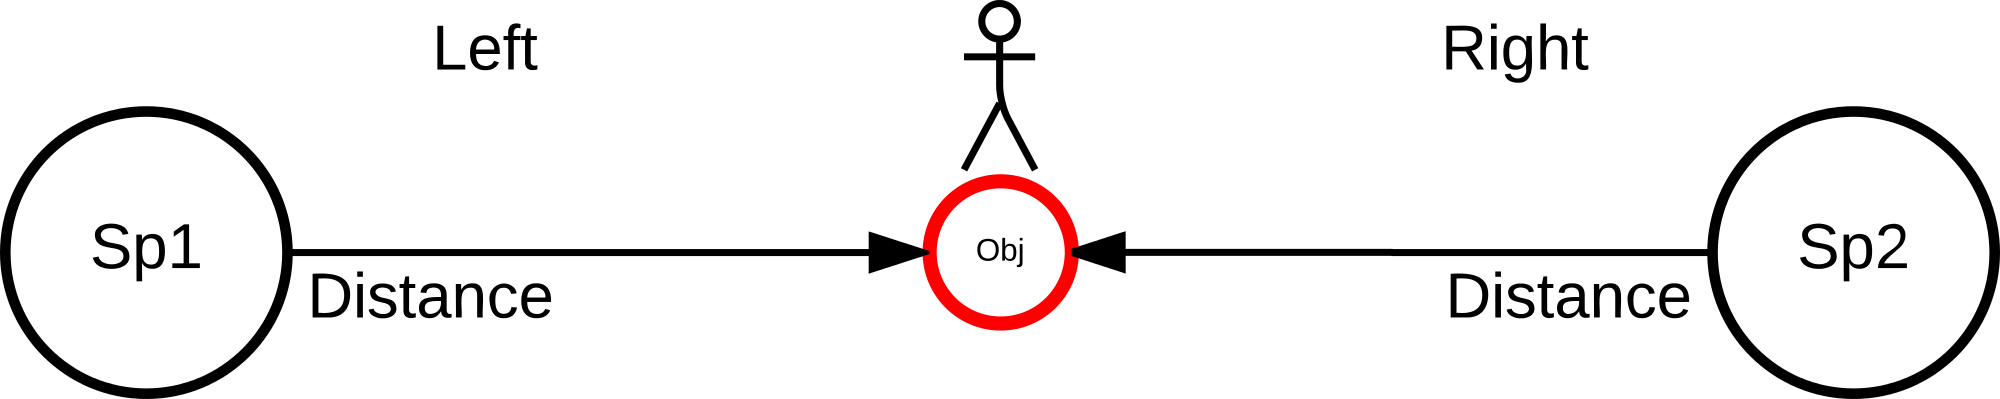
\includegraphics[width=.8\textwidth]{client_rwf_center}
    \caption{Virtual object at center}
    \label{fig:client_rwf_center}
\end{figure}

In figure \ref{fig:client_rwf_offset} is the next example. Now the virtual object is at an offset from the user.
you would normally say that \say{Sp1} has a shorter distance and \say{Sp2} has a greater distance.
To compensate, \say{Sp2} needs to be harder then \say{Sp1}. Let's think about this for a minute.
If the user is standing in the middle and \say{Sp2} is playing harder then \say{Sp1}.
This means that the \say{Right} side produces more sound then the \say{Left} side.
The user would hear more sound coming from the \say{Right} side, so the user would think that the sound comes from the \say{Right} side.

\begin{figure}[H]
    \centering
    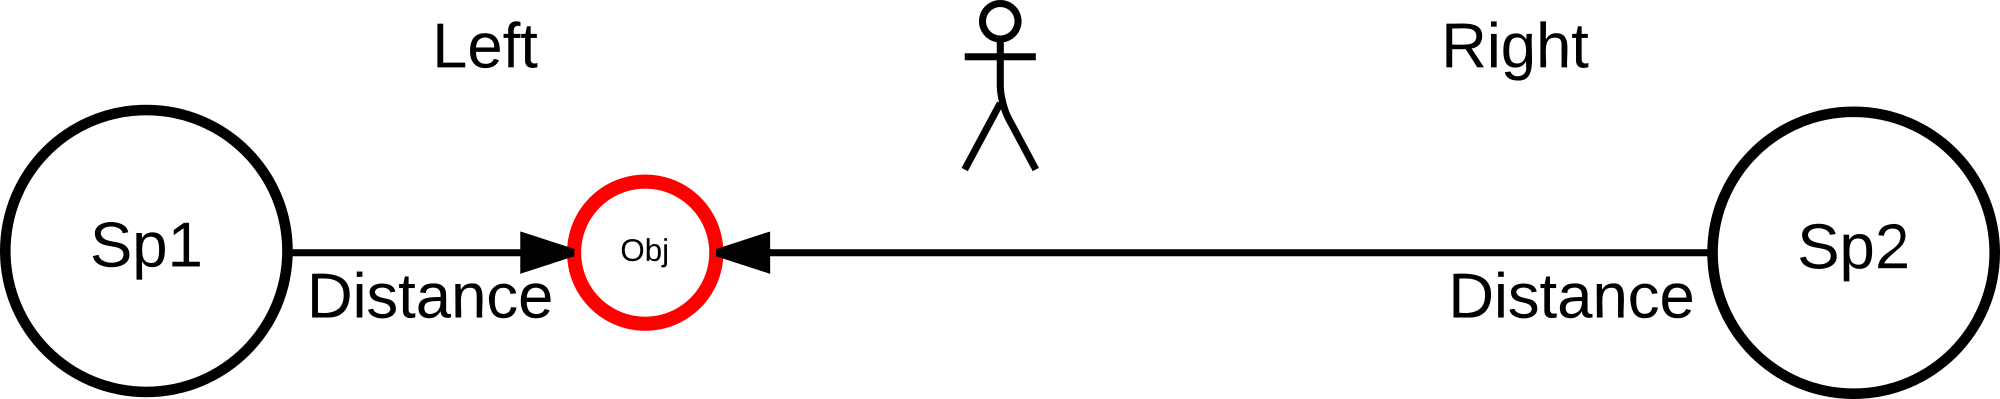
\includegraphics[width=.8\textwidth]{client_rwf_offset}
    \caption{Virtual object at offset}
    \label{fig:client_rwf_offset}
\end{figure}

In conclusion the speaker where the object is closest to, needs to produce the most sound.

\subsection{Calculating the RWF}
\label{sub:client_calculating_the_rwf}
It's is clear that the speaker closest to the object, needs to produce more sound.
This way, of the user stands in the middle he will think that the sound is coming from the place where the sound is the hardest.

The value of the volume in this project, is called the relative weight factor or RWF in short.
Because there needs to be a value that represents the relative weight each speaker has relative to any object.
Table \ref{table:client_calculate_rwf_for_three_speakers_1_2_3} shows the calculation of the RWF for three objects.


In the left half of the table are the speakers with there distances to an object.
The units of measurement don't matter in this case, as long as they are of the same type.
The first step is to \say{invert} all the distances. See the table \ref{table:client_calculate_rwf_for_three_speakers_1_2_3} \say{Inverse distance}.
This is done by adding all the distances and subtracting the distance of a speaker to an object from this total.
Next there are the values at the bottom of the table. The \textit{Head} is the maximal value of the RWF factor.
The \textit{tail} is the minimal value of the RWF factor. In this project's case, this would be a value between 0\% and 100\%.
Now the number of steps are known.(head-tail)
To get the actual RWF value the \say{value per step} is needed. This is calculated by dividing the \say{value per step} by the total inverse distance value.
Now it is a matter of multiplying the inverse distance with the \say{value per step} and the RWF values are known.

\newcommand\RWFTable[3]% #1 = distance speaker 1, #2 = distance speaker 2, #3 = distance speaker 3
{\begin{table}[H]
    \renewcommand{\familydefault}{\ttdefault}\nimbus
    \centering
    \begin{spreadtab}{{tabular}{ l | r || r l l | r l l }}
        @Speaker    & @Distance                             & @\multicolumn{3}{c|}{Inverse distance}& @\multicolumn{3}{c}{Calculated Value} \\
        @A          & #1                                    & :={b5}&-:={b2}&= :={b5-b2}            & :={e2}&*:={e10}       &= :={round(e2*(e9/e5), 0)} \\
        @B          & #2                                    & :={b5}&-:={b3}&= :={b5-b3}            & :={e3}&*:={e10}       &= :={round(e3*(e9/e5), 0)} \\
        @C          & #3                                    & :={b5}&-:={b4}&= :={b5-b4}            & :={e4}&*:={e10}       &= :={round(e4*(e9/e5), 0)} \\ \hline
        @Total:     & sum(b2:b4)                            &       &       &= :={sum(e2:e4)}       & @\multicolumn{2}{c}{} &= :={sum(h2:h4)}\\ \hline \hline
                    &                                       &       &       &                       & \\
        @\multicolumn{2}{r ||}{Head}                        & 100   &       &                       & \\
        @\multicolumn{2}{r ||}{Tail}                        & 0     &       &                       & \\
        @\multicolumn{2}{r ||}{Volume steps [head-tail]}    & :={c7}&-:={c8}& = :={c7-c8}           & \\
        @\multicolumn{2}{r ||}{Value per volume step}       & :={e9}&/:={e5}& = :={round(e9/e5, 2)} & \\
    \end{spreadtab}
    \caption{Calculate RWF for three speakers. Distances: #1, #2 and #3}
    \label{table:client_calculate_rwf_for_three_speakers_#1_#2_#3}
\end{table}
}

\RWFTable{1}{2}{3} % print RWF Table

The tables below show other examples with different distances values.
(See table \ref{table:client_calculate_rwf_for_three_speakers_1_1_1} and \ref{table:client_calculate_rwf_for_three_speakers_5_8_3})

\RWFTable{1}{1}{1} % print RWF Table

\RWFTable{5}{8}{3} % print RWF Table

\section{Logger}
\label{sec:client_logger}
Logger
